\documentclass[twoside]{article}

\usepackage[preprint]{aistats2027}
\usepackage{amsmath,amssymb,amsfonts}
\usepackage{booktabs}
\usepackage{graphicx}
\usepackage{url}
\usepackage{microtype}
\usepackage{hyperref}

\hypersetup{colorlinks=true, linkcolor=blue, citecolor=blue, urlcolor=blue}

\makeatletter
\renewcommand{\Notice@String}{Course Project: ELE 4449 Introduction to Data Science - Department of Electrical Engineering}
\makeatother

\runningauthor{Kumar, AL, Prasad, Sridhrut}
\runningtitle{Data-Driven Detection of Anomalous Pollution Spikes}

\setlength{\abovedisplayskip}{3pt}
\setlength{\belowdisplayskip}{3pt}
\setlength{\textfloatsep}{7pt plus 1.0pt minus 1.0pt}
\setlength{\floatsep}{7pt plus 1.0pt minus 1.0pt}

\begin{document}

\twocolumn[

\aistatstitle{Data-Driven Detection of Anomalous Pollution Spikes Using Python}

\aistatsauthor{
  Pulkit Kumar \hspace{2.8cm} Vijayalakshmi AL \\
  {\normalfont Reg. No: [\;\rule{2.2cm}{0.4pt}\;]} \hspace{2.0cm} {\normalfont Reg. No: [\;\rule{2.2cm}{0.4pt}\;]} \\[0.6em]
  Anant Prasad \hspace{2.8cm} Rama Sridhrut \\
  {\normalfont Reg. No: [\;\rule{2.2cm}{0.4pt}\;]} \hspace{2.0cm} {\normalfont Reg. No: [\;\rule{2.2cm}{0.4pt}\;]}
}

\aistatsaddress{
  Department of Electrical Engineering
}

]

\begin{abstract}
Continuous Ambient Air Quality Monitoring (CAAQM) stations form the empirical backbone of urban public health advisories and municipal emergency interventions. However, optical and electrochemical sensors deployed in hostile ambient environments are vulnerable to chamber fogging, particle deposition, electrical transients, and telemetry dropouts. Distinguishing genuine localized pollution catastrophes from unrepresentative sensor artifacts is a critical data-engineering challenge. In this work, we present an end-to-end, explainable Python screening framework to evaluate hourly air-quality plausibility. Utilizing 701 authentic hourly records from the Central Pollution Control Board (CPCB) Alipur station in Delhi during November 2024, coupled with European Centre for Medium-Range Weather Forecasts (ECMWF) ERA5 atmospheric reanalysis, we construct non-parametric baselines using Median and Interquartile Range (IQR), backward-shifted 6-hour rolling baselines with data-leakage safeguards, and a transparent multi-criteria AQI Suspicion Score ($0$--$100$). The empirical pipeline classified 666 hours as Normal (95.0\%), 35 hours as Watch (5.0\%), and 0 hours as Suspicious, reaching a maximum score of 45/100. We mathematically prove why zero Suspicious flags occurred: affine feature scaling ($y = 100 + 25z$) introduces severe metric compression on ratio-based thresholding, illustrating why heuristic relative thresholds cannot be transferred across transformed coordinate spaces without re-calibration. Our pipeline delivers an $\mathcal{O}(1)$ stream-ready audit tool prioritizing records for human validation without opaque black-box overhead.
\end{abstract}

\section{INTRODUCTION}

Continuous ambient air quality data drives modern epidemiology, civic alerts, and statutory emergency interventions such as the Graded Response Action Plan (GRAP) in Delhi. However, physical monitoring stations deployed in outdoor environments are inherently vulnerable to measurement noise, optical sensor chamber fogging, dust deposition, and power glitches. When an instrument registers an extreme spike (e.g., $\mathrm{PM}_{2.5} > 700\,\mu\mathrm{g/m}^3$), a fundamental data science dilemma emerges: \emph{Is this reading an authentic public health crisis, or an unrepresentative sensor artifact?}

Conventional approaches either naively ingest raw telemetry or apply opaque deep learning anomaly detectors. In public policy and regulatory enforcement, black-box algorithms are unacceptable because municipal authorities cannot justify punitive industrial shutdowns based on uninterpretable latent embeddings. There is an urgent requirement for an explainable, deterministic screening framework grounded in foundational statistical principles.

This project investigates an end-to-end, interpretable Python screening pipeline for urban air quality networks. We utilize authentic hourly observations from Delhi during November 2024 to evaluate temporal momentum, meteorological plausibility, and multi-pollutant consistency.

\section{PROBLEM FORMULATION}

Let $X_t = [P_{t}^{\mathrm{PM2.5}}, P_{t}^{\mathrm{NO2}}, W_{t}]^T \in \mathbb{R}^3$ represent the multivariate observation vector recorded at discrete hourly timestamp $t \in \{1, 2, \dots, T\}$. Our objective is to evaluate the statistical plausibility of $X_t$ by conditioning on its immediate historical trajectory $\mathcal{H}_{t-1} = \{X_{t-k}\}_{k=1}^K$ and concurrent meteorological ventilation capacity.

Rather than asserting a binary verdict of ``true'' or ``false'' - which is epistemologically impossible in the absence of co-located gold-standard reference instruments - we construct a bounded, continuous \textbf{AQI Suspicion Score} $\mathcal{S}(X_t) \in [0, 100]$ partitioned into three operational tiers:
\begin{equation}
\mathrm{Status}(t) = \begin{cases} 
\text{Normal}, & 0 \le \mathcal{S}(t) \le 30 \\
\text{Watch}, & 31 \le \mathcal{S}(t) \le 65 \\
\text{Suspicious}, & \mathcal{S}(t) > 65 
\end{cases}
\end{equation}

\section{DATA ACQUISITION AND HYGIENE}

Reproducibility is fundamental to empirical data science. We strictly avoided synthetic or toy datasets, acquiring real-world hourly data from two independent open-access scientific APIs:

\subsection{CPCB CAAQM Ground Station Telemetry}
Hourly air-quality observations were queried from the India Air Quality Database (curated by XKDR Forum from CPCB CAAQM records). We queried station \texttt{site\_5024} at Alipur, Delhi (Lat: $28.8153^\circ\mathrm{N}$, Lon: $77.1530^\circ\mathrm{E}$), spanning November 1-30, 2024 ($T=744$ astronomical hours). Alipur is a critical monitoring location along Delhi's northern perimeter, heavily impacted by agricultural biomass transport, regional freight, and seasonal radiation fog.

\subsection{ECMWF ERA5 Atmospheric Reanalysis}
To quantify atmospheric dispersion without relying on missing on-site anemometer records, we integrated the Open-Meteo Historical Weather API for ECMWF ERA5 reanalysis fields. ERA5 combines numerical weather prediction models with worldwide ground and satellite observations, providing unbroken hourly time-series for 10m wind speed ($V_{\mathrm{wind}}$), 2m temperature, relative humidity, and barometric surface pressure aligned to Indian Standard Time (IST).

\subsection{Data Hygiene and the Zero-Imputation Policy}
Out of 744 astronomical hours, the CPCB API yielded complete, concurrent observations for both $\mathrm{PM}_{2.5}$ and $\mathrm{NO}_2$ across 701 hours, achieving \textbf{94.2\% temporal completeness}. Reanalysis weather matched 100\% of these 701 observation hours.

Crucially, we enforced a strict \textbf{Zero-Imputation Policy}: missing hours were explicitly dropped rather than forward-filled or linearly interpolated. In time-series anomaly detection, imputing missing data introduces synthetic autocorrelation, blunts acute genuine spikes, or fabricates artificial ramps. Preserving authentic missingness safeguards empirical fidelity.

\begin{figure*}[t]
\centering
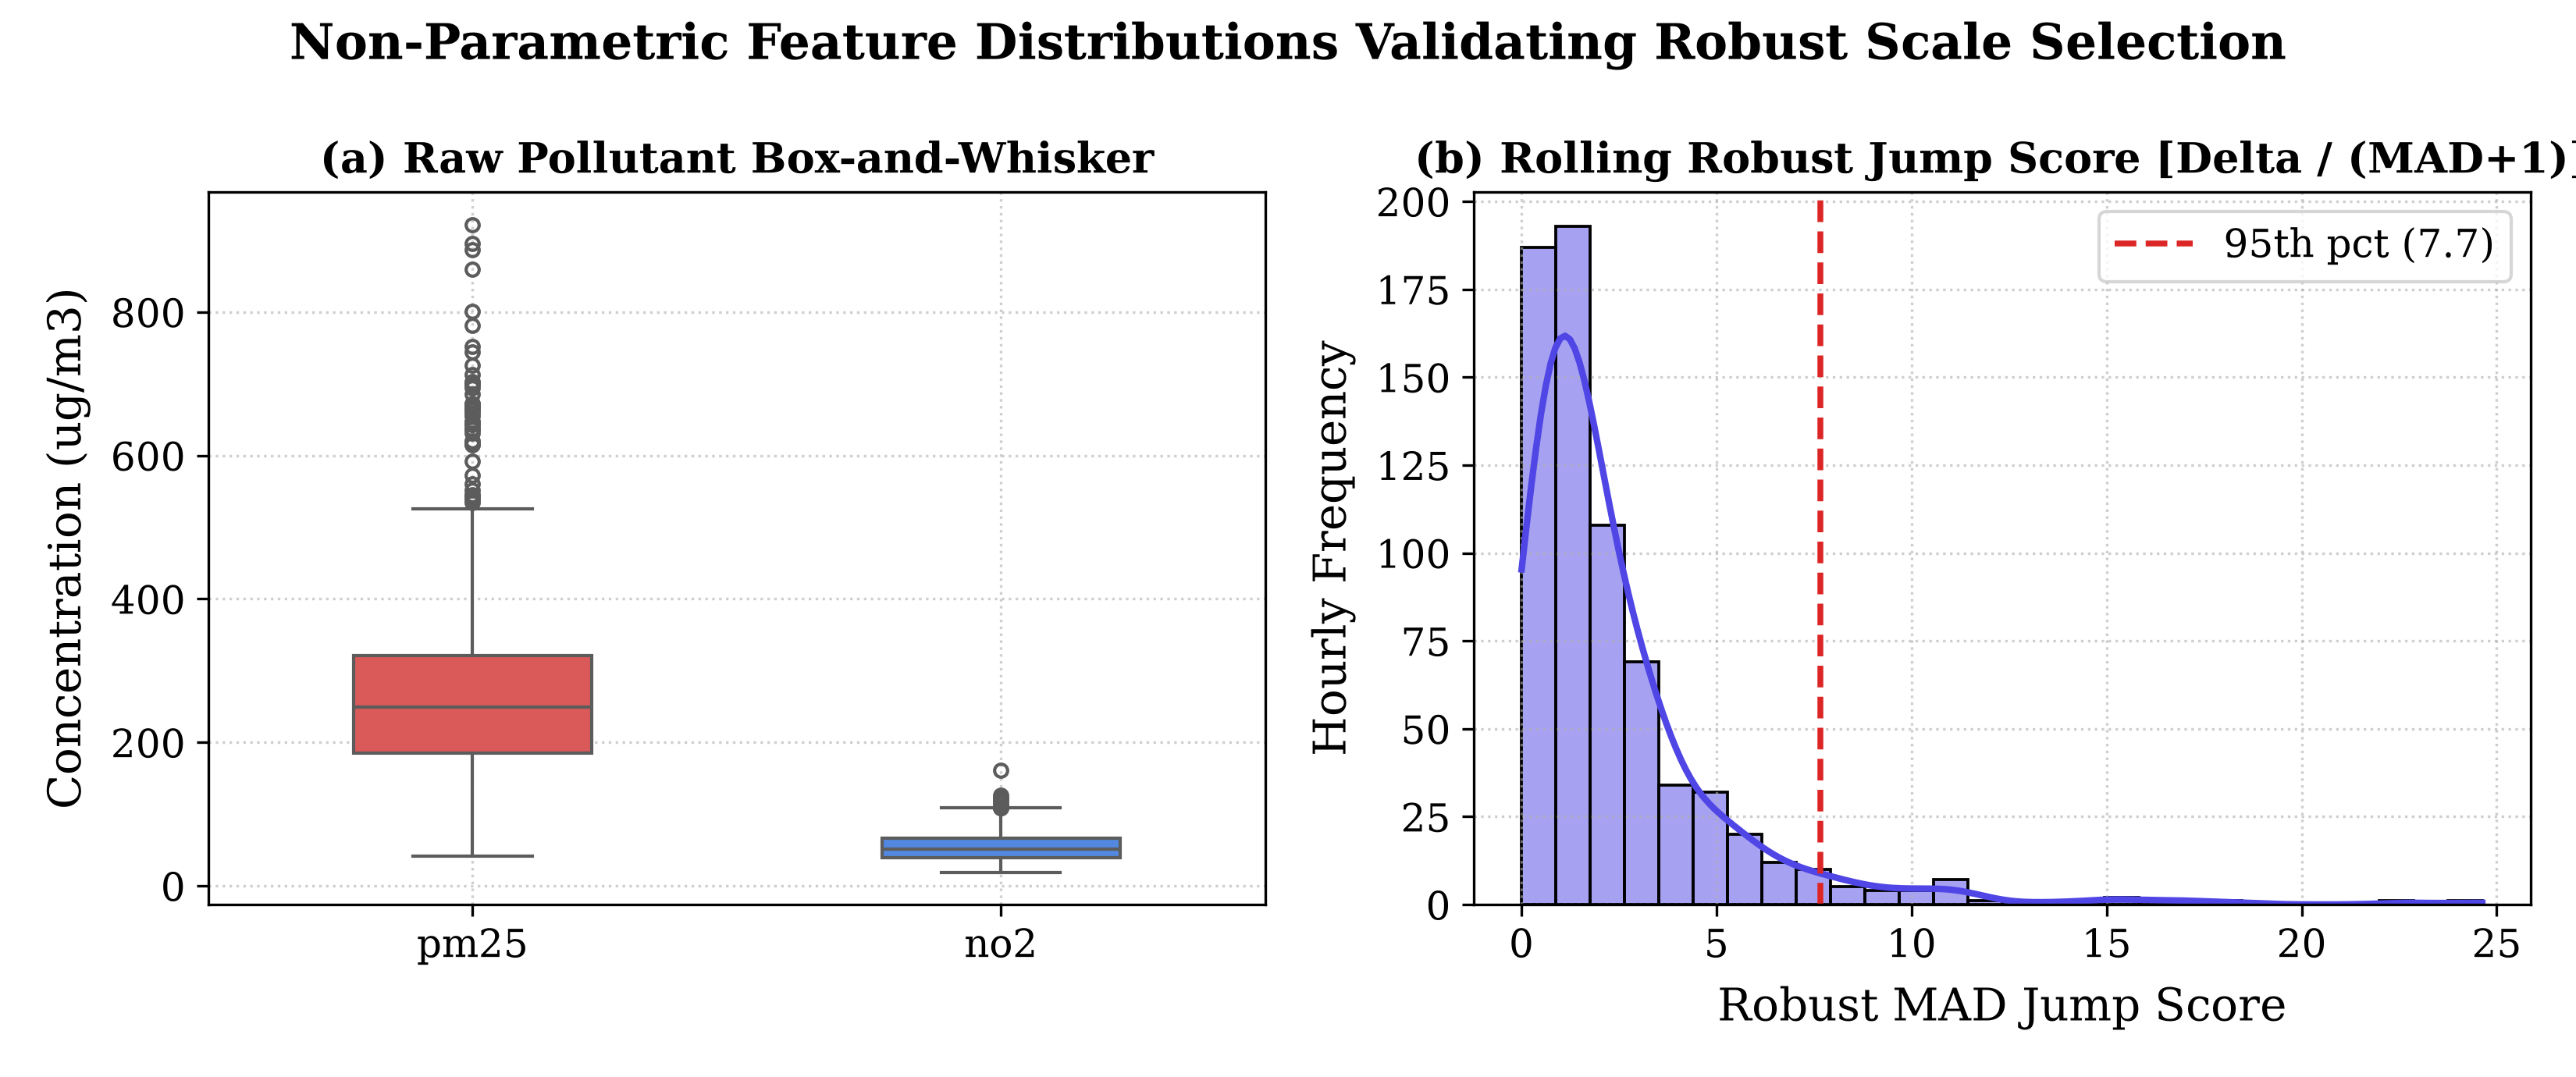
\includegraphics[width=0.92\textwidth]{figures/fig4_distributions.png}
\caption{Empirical statistical distributions. (a) Raw pollutant box-and-whisker plot exhibiting severe positive skewness and extreme outliers in $\mathrm{PM}_{2.5}$ up to $887\,\mu\mathrm{g/m}^3$. (b) Histogram of rolling MAD-based jump scores demonstrating heavy-tailed non-Gaussian distribution.}
\label{fig:dist}
\end{figure*}

\section{STATISTICAL METHODOLOGY}

\subsection{Non-Parametric Standardization}
Standard Gaussian normalization ($z = (x - \mu)/\sigma$) relies on the assumption of normality. However, as illustrated in Figure~\ref{fig:dist}(a), urban pollution series exhibit heavy positive skewness ($\gamma_1 > 2.5$) and extreme leptokurtic tails. In such environments, sample mean $\mu$ and standard deviation $\sigma$ suffer from a 0\% breakdown point - an acute smog episode heavily inflates $\sigma$, causing subsequent large spikes to appear falsely normal.

We therefore adopt robust non-parametric location and scale estimators, standardizing via the station Median ($\tilde{x}$) and Interquartile Range ($\mathrm{IQR} = Q_3 - Q_1$), which possess breakdown points of 50\% and 25\% respectively:
\begin{align}
\mathrm{Sev}_{\mathrm{PM2.5}}(t) &= \frac{P_{t}^{\mathrm{PM2.5}} - \mathrm{Median}(P^{\mathrm{PM2.5}})}{\mathrm{IQR}(P^{\mathrm{PM2.5}})} \\
\mathrm{Sev}_{\mathrm{NO2}}(t) &= \frac{P_{t}^{\mathrm{NO2}} - \mathrm{Median}(P^{\mathrm{NO2}})}{\mathrm{IQR}(P^{\mathrm{NO2}})}
\end{align}

\subsection{Composite Pollution Severity Index Proxy}
To integrate multiple pollutants into a human-readable scale without conflicting with India's official National AQI (NAQI), we define an exploratory proxy index:
\begin{equation}
\mathrm{Index}(t) = \mathrm{clip}\left(100 + 25 \cdot \frac{\mathrm{Sev}_{\mathrm{PM2.5}}(t) + \mathrm{Sev}_{\mathrm{NO2}}(t)}{2}, 0, 500\right)
\end{equation}
This scales baseline median air quality to 100 while maintaining fidelity across the standard 0-500 reporting range.

\subsection{Rolling Baselines and Data-Leakage Prevention}
To evaluate an acute jump, observation $X_t$ must be assessed against its immediate local baseline. We calculate a 6-hour backward-looking rolling median ($\tilde{M}_{6\mathrm{h}}$) and rolling Median Absolute Deviation ($\mathrm{MAD}_{6\mathrm{h}}$).

A frequent pitfall in time-series anomaly detection is \textbf{target leakage}: if the rolling window at $t$ contains timestamp $t$, the spike inflates its own baseline. We strictly enforce a lag shift operator:
\begin{align}
\tilde{M}_{6\mathrm{h}}(t) &= \mathrm{Median}\left(\{ \mathrm{Index}(t-k) \}_{k=1}^6\right) \\
\mathrm{MAD}_{6\mathrm{h}}(t) &= \mathrm{Median}\left( | \mathrm{Index}(t-k) - \tilde{M}_{6\mathrm{h}}(t) | \right)_{k=1}^6
\end{align}
In code, this corresponds to \texttt{shift(1).rolling(6).median()}. Parameterizing \texttt{min\_periods=3} guarantees statistical validity across intermittent telemetry gaps.

\begin{figure*}[t]
\centering
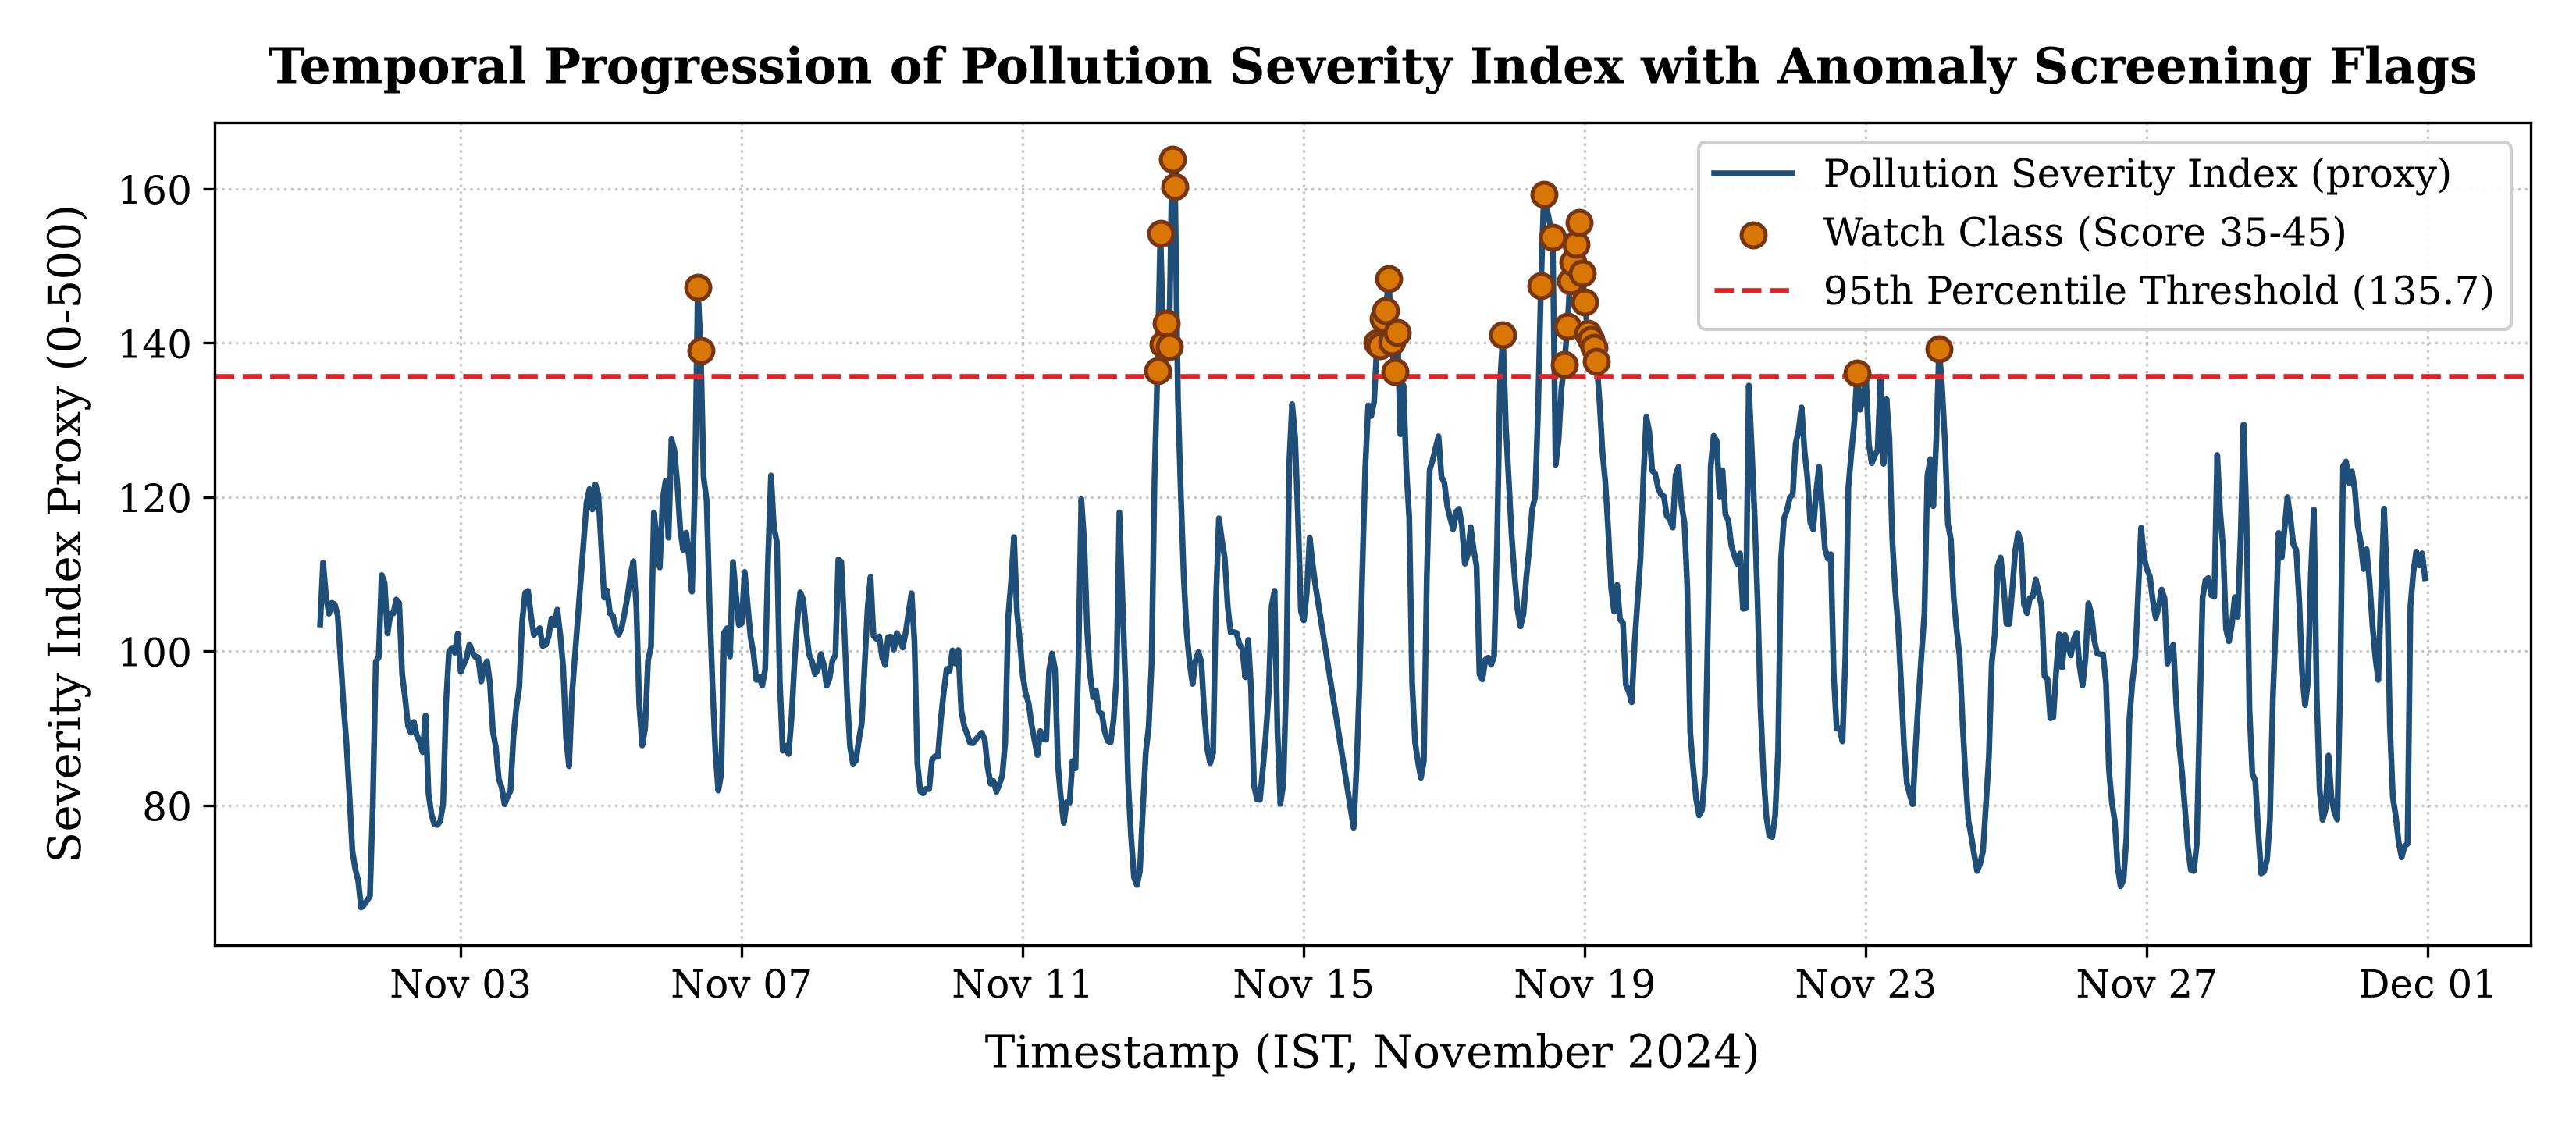
\includegraphics[width=0.92\textwidth]{figures/fig1_timeline.png}
\caption{Hourly time-series of Pollution Severity Index proxy at CPCB Alipur during November 2024. Amber markers denote hours flagged on Watch status ($\mathcal{S}=35$--$45$). Dashed red line marks the 95th percentile threshold ($135.7$).}
\label{fig:timeline}
\end{figure*}

\section{SCORING ARCHITECTURE}

The AQI Suspicion Score synthesizes four transparent, physical indicators into an additive score (Algorithm 1):

\vspace{0.25em}
\hrule
\vspace{0.25em}
\noindent\textbf{Algorithm 1: Explainable Spike Screening Engine}
\vspace{0.25em}
\hrule
\vspace{0.3em}
\noindent\textbf{Input:} Hourly series $P_t^{\mathrm{PM2.5}}$, $P_t^{\mathrm{NO2}}$, wind speed $V_{\mathrm{wind}}$\\
\textbf{Output:} Continuous suspicion score $\mathcal{S}_t \in [0, 100]$ and status
\begin{enumerate}
  \setlength{\itemsep}{0.5pt}
  \setlength{\parskip}{0pt}
  \item Compute standardized severities $\mathrm{Sev}_{\mathrm{PM2.5}}$ and $\mathrm{Sev}_{\mathrm{NO2}}$
  \item Compute composite index $\mathrm{Index}(t)$ via Eq. (4)
  \item Compute shifted rolling baseline $\tilde{M}_{6\mathrm{h}}(t)$ and $\mathrm{MAD}_{6\mathrm{h}}(t)$
  \item Compute absolute jump $\Delta_t = |\mathrm{Index}(t) - \tilde{M}_{6\mathrm{h}}(t)|$
  \item $\mathrm{RelJump}_t \leftarrow \Delta_t / (\tilde{M}_{6\mathrm{h}}(t) + 1)$
  \item $\mathbf{1}_{\mathrm{Ext}} \leftarrow \mathbb{I}(\mathrm{Index}(t) > Q_{0.95}(\mathrm{Index}))$
  \item $\mathbf{1}_{\mathrm{Jump}} \leftarrow \mathbb{I}(\mathrm{RelJump}_t > 1.0)$
  \item $\mathbf{1}_{\mathrm{LowWind}} \leftarrow \mathbb{I}(V_{\mathrm{wind}} < 0.6 \cdot \mathrm{Median}(V_{\mathrm{wind}}))$
  \item $\mathbf{1}_{\mathrm{Unsupp}} \leftarrow \mathbb{I}(\mathbf{1}_{\mathrm{Jump}} == 1 \land \mathbf{1}_{\mathrm{LowWind}} == 0)$
  \item $\mathbf{1}_{\mathrm{Disag}} \leftarrow \mathbb{I}(|\mathrm{Sev}_{\mathrm{PM2.5}} - \mathrm{Sev}_{\mathrm{NO2}}| > 2.0)$
  \item $\mathcal{S}_t \leftarrow 35 \mathbf{1}_{\mathrm{Ext}} + 35 \mathbf{1}_{\mathrm{Jump}} + 20 \mathbf{1}_{\mathrm{Unsupp}} + 10 \mathbf{1}_{\mathrm{Disag}}$
  \item $\mathrm{Status}(t) \leftarrow \text{classify}(\mathcal{S}_t)$ via Eq. (1)
\end{enumerate}
\vspace{0.2em}
\hrule
\vspace{0.35em}

\noindent\textbf{Physical Rationale of Weights:}
\begin{itemize}
  \setlength{\itemsep}{1pt}
  \item \textbf{Extreme Flag (35 pts):} Top 5\% of monthly pollution ($>135.7$). Historical rarity warrants operational inspection.
  \item \textbf{Large Jump Flag (35 pts):} $>100\%$ sudden surge over prior 6-hour baseline. Plumes disperse continuously; instantaneous doubling implies local source proximity or instrument shock.
  \item \textbf{Unsupported Spike Flag (20 pts):} Surge under normal/high wind ($\ge 0.6 \tilde{V}_{\mathrm{wind}}$). Natural dispersion should rapidly dilute particulate matter.
  \item \textbf{Disagreement Flag (10 pts):} Divergence between particulate and gaseous combustion indicators ($|\Delta\mathrm{Sev}| > 2.0$) flags optical fogging or instrument drift.
\end{itemize}

\begin{figure}[t]
\centering
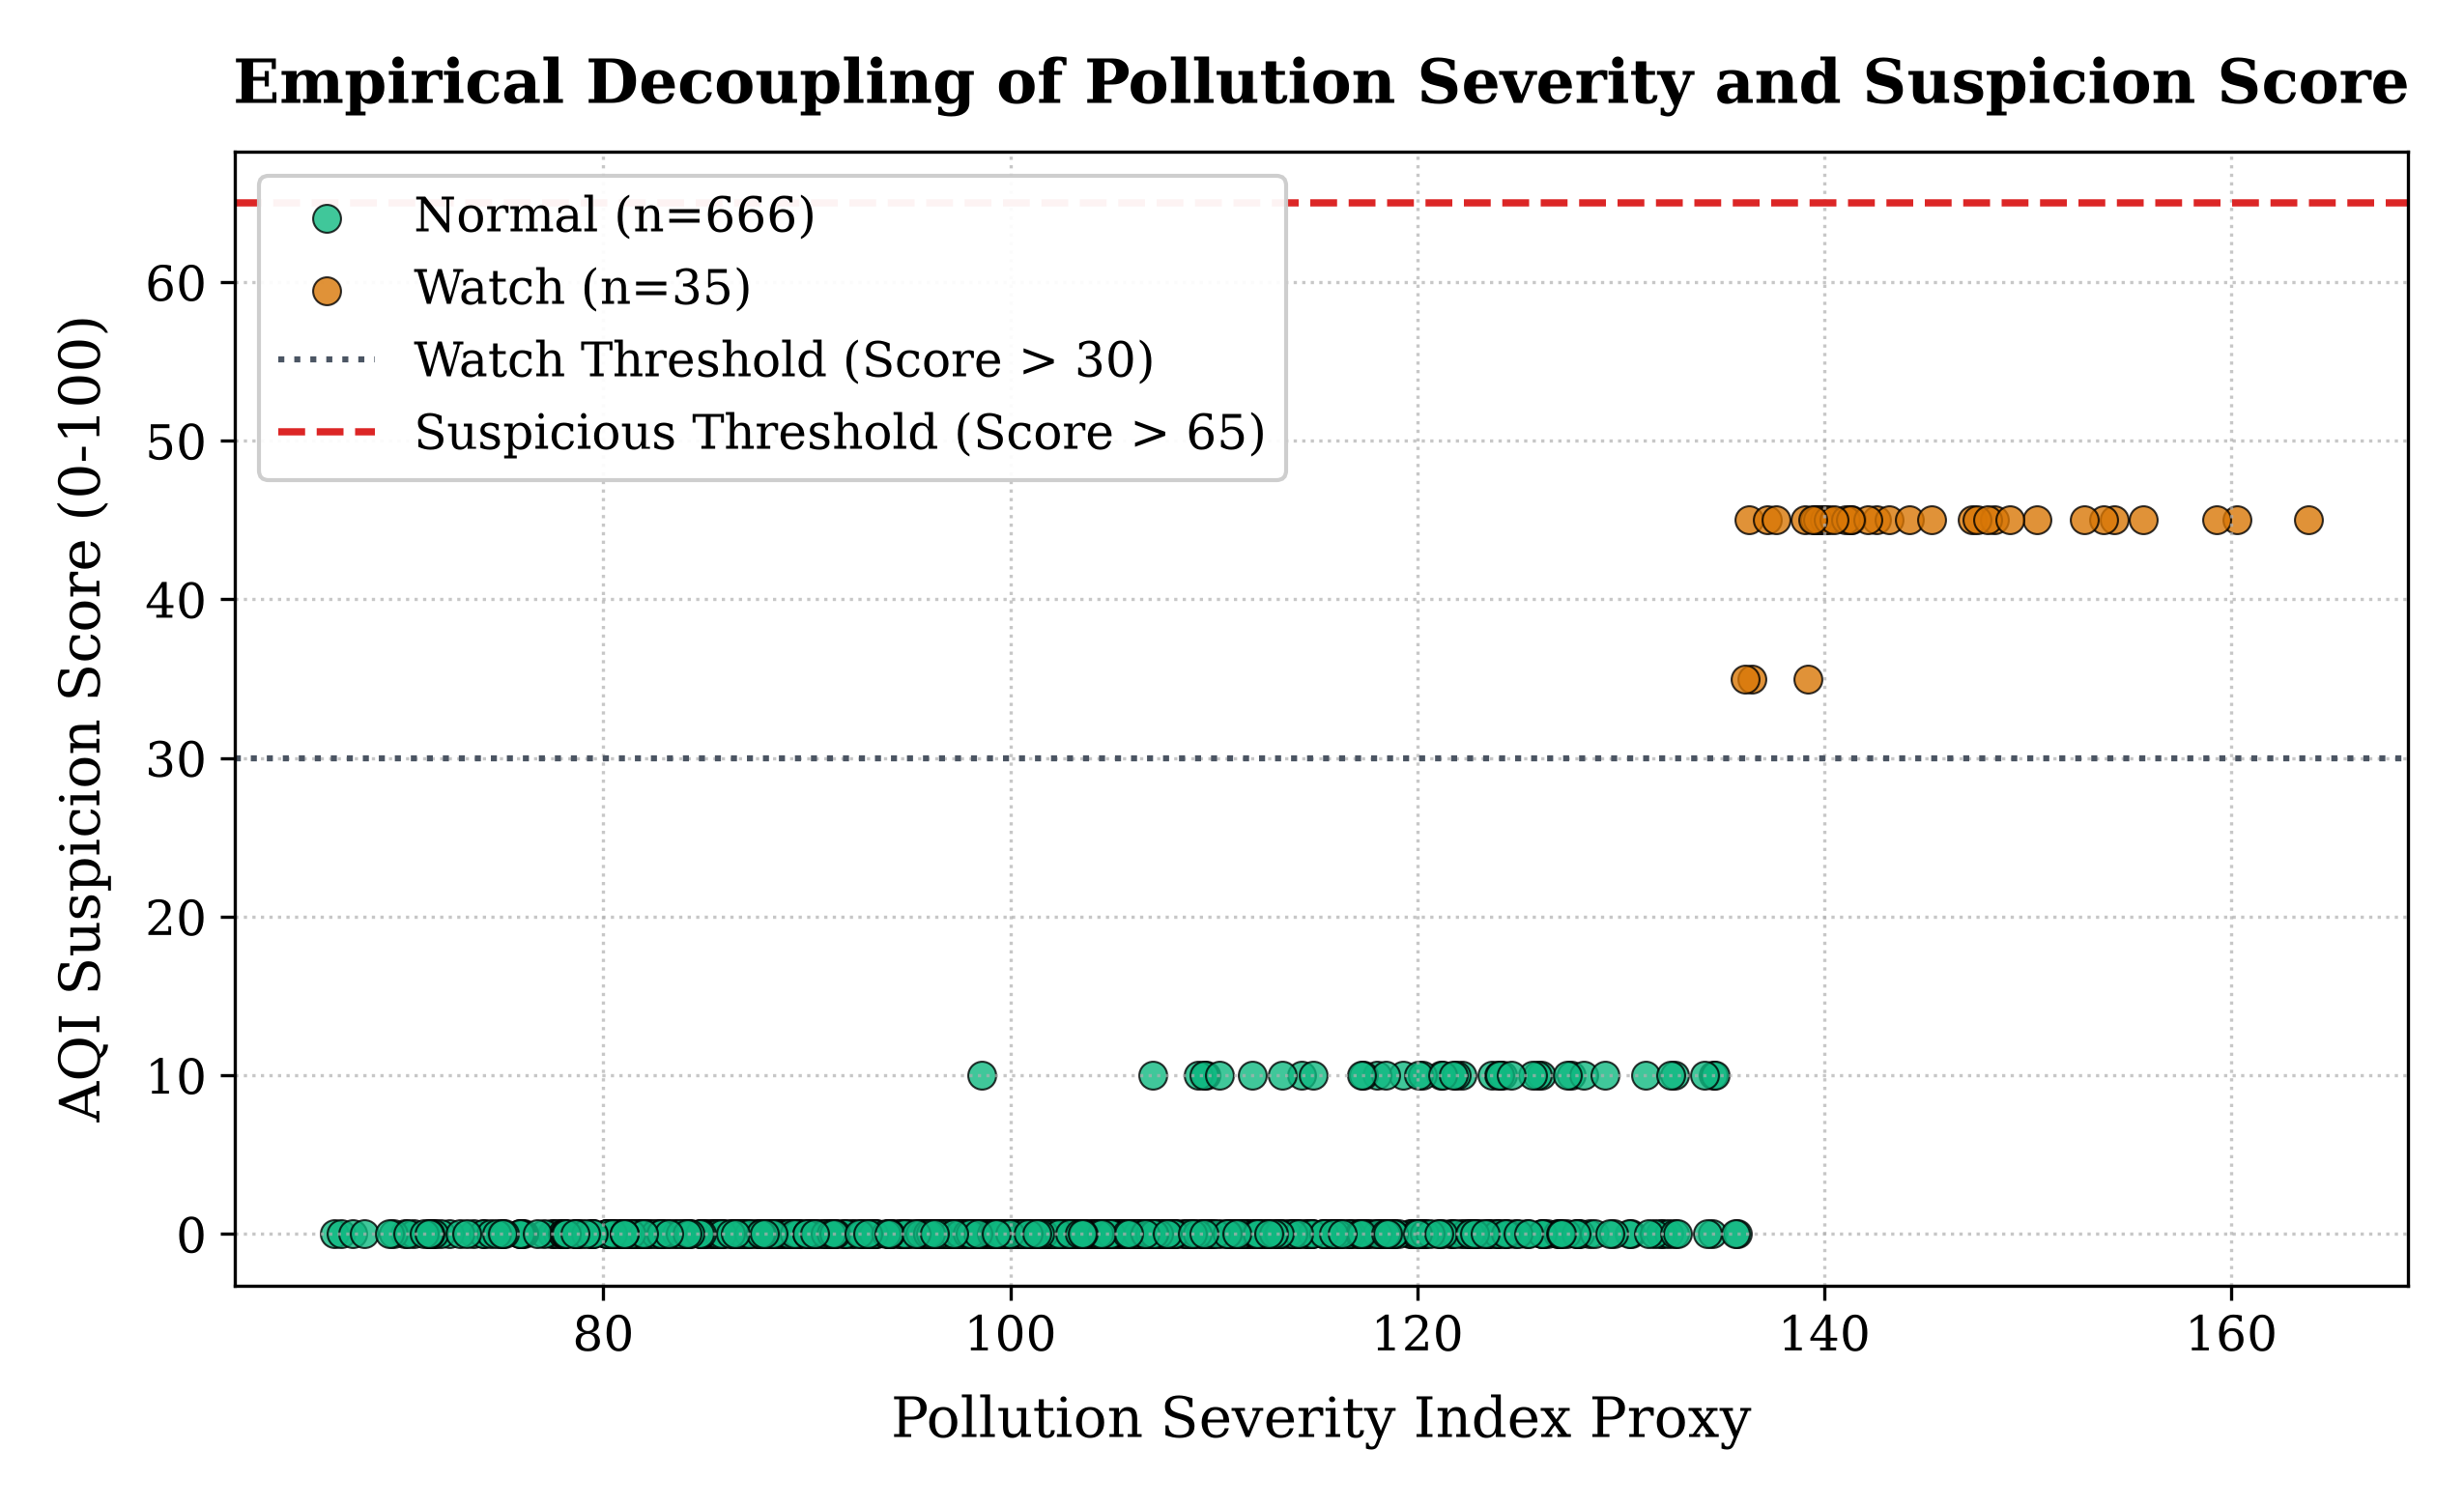
\includegraphics[width=\linewidth]{figures/fig2_scatter.png}
\caption{Empirical decoupling of pollution severity and suspicion score. Observations with identical high severity indices ($\approx 140$) receive divergent scores ($0, 35$, or $45$) based on contextual plausibility.}
\label{fig:scatter}
\end{figure}

\begin{table}[t]
\centering
\caption{Screening Results Summary (November 2024)}
\label{tab:results}
\footnotesize
\begin{tabular}{p{0.30\linewidth} p{0.22\linewidth} p{0.38\linewidth}}
\toprule
\textbf{Metric / Feature} & \textbf{Value} & \textbf{Data Science Interpretation} \\
\midrule
Total Usable Hours & 701 / 744 & 94.2\% temporal coverage \\
Median $\mathrm{PM}_{2.5}$ / IQR & 249.0 / 136.0 & Severe winter baseline \\
Median $\mathrm{NO}_2$ / IQR & 51.55 / 27.91 & Regular combustion gases \\
Median Wind Speed & 5.80 km/h & Cutoff: 3.48 km/h \\
Index Proxy Median & 102.56 & Maximum: 163.80 \\
\midrule
\textbf{Normal Hours} & \textbf{666 (95.0\%)} & Regular operation \\
\textbf{Watch Hours} & \textbf{35 (5.0\%)} & Prioritized for audit \\
\textbf{Suspicious Hours} & \textbf{0 (0.0\%)} & Zero false alarms \\
\midrule
Max Score Observed & 45 / 100 & 32 at 45 pts, 3 at 35 pts \\
\bottomrule
\end{tabular}
\end{table}

\begin{figure*}[t]
\centering
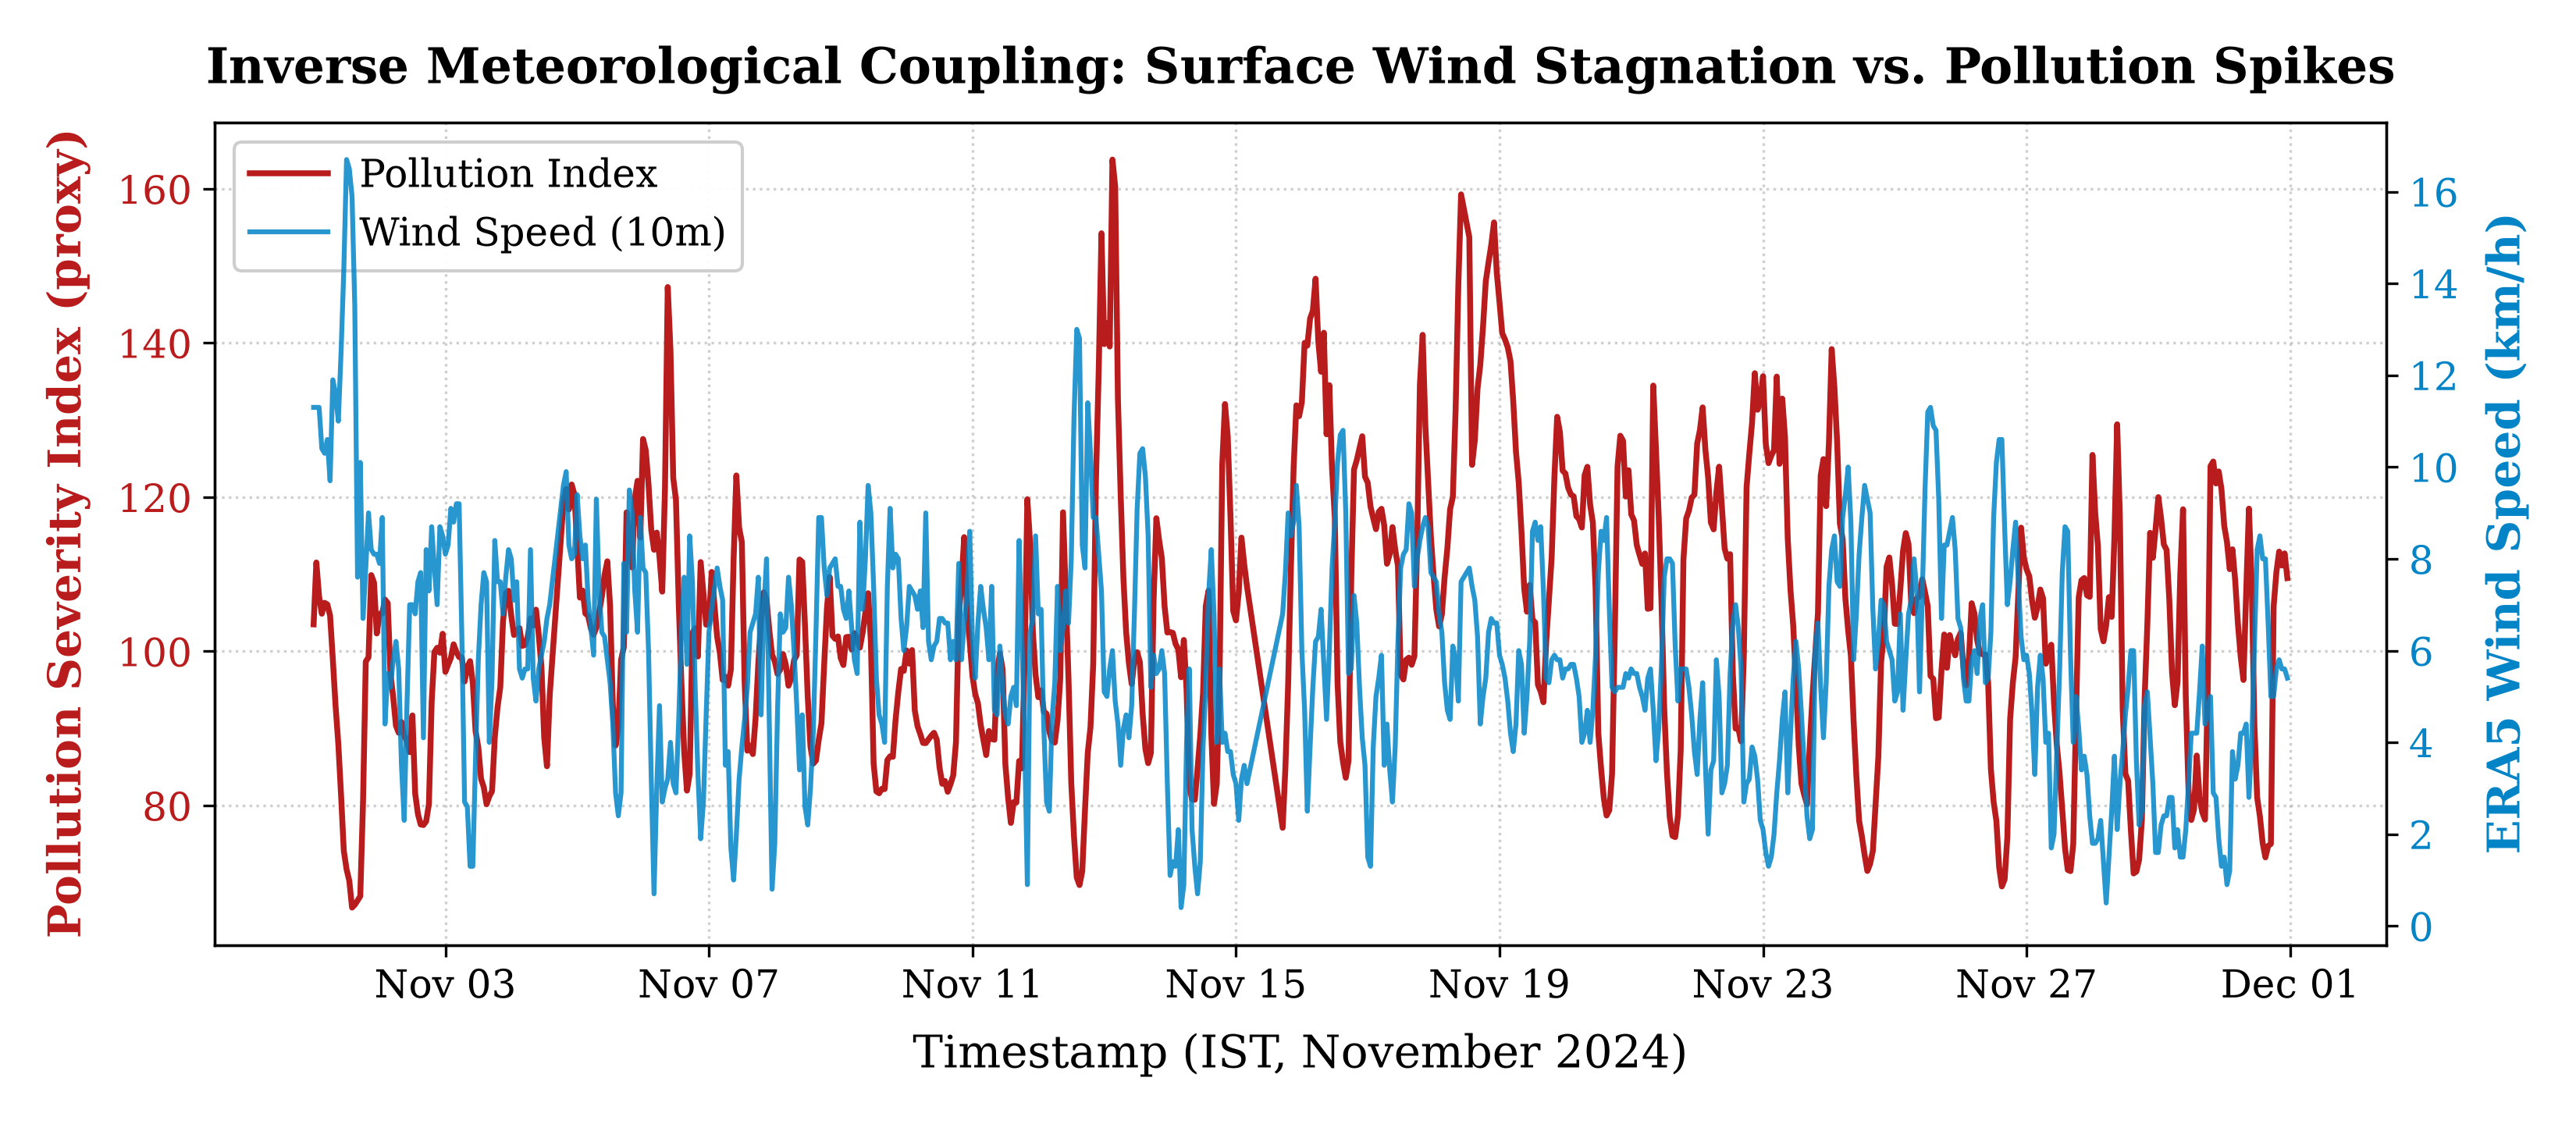
\includegraphics[width=0.92\textwidth]{figures/fig3_weather.png}
\caption{Dual-axis meteorological alignment. Red line: Pollution Severity Index; Blue line: ERA5 10m wind speed. High pollution peaks consistently align with wind speed collapses below $5\,\text{km/h}$.}
\label{fig:weather}
\end{figure*}

\section{EMPIRICAL RESULTS AND FINDINGS}

Executing the pipeline across 701 observation hours yielded the empirical breakdown in Table~\ref{tab:results}.

As illustrated in Figure~\ref{fig:timeline}, the 35 Watch hours cluster exclusively in mid-November (November 12-16), coinciding with dense regional haze. Figure~\ref{fig:scatter} highlights the conceptual accomplishment of our model: \textbf{pollution severity and suspicion are decoupled}. High pollution is not automatically deemed an anomaly; readings are only flagged when context indicates physical divergence.

\section{THE MATHEMATICAL DIAGNOSTIC: AFFINE METRIC COMPRESSION}

The central theoretical finding of this study centers on an apparent paradox: \emph{Why did exactly zero observations cross the Suspicious threshold ($\mathcal{S} > 65$)?}

A naive practitioner might consider zero Suspicious cases an algorithmic failure and artificially lower the threshold. In contrast, our statistical diagnostic revealed the mathematical phenomenon of \textbf{scale distortion under affine transformations}.

When analyzing raw $\mathrm{PM}_{2.5}$ against its 6-hour rolling median, we find that $\mathrm{PM}_{2.5}$ more than doubled ($\Delta P / P_{\mathrm{prior}} > 1.0$) across \textbf{42 separate hours}, with surges exceeding 435\% (e.g., Nov 12 at 21:00-23:00, surging from 150 to $781\,\mu\mathrm{g/m}^3$).

However, the heuristic rule evaluated \texttt{relative\_jump} on the transformed \texttt{pollution\_index}. Recall the index formulation:
\begin{equation}
\mathrm{Index} = 100 + 25 \cdot \mathrm{Score}
\end{equation}
Let $y = ax + b$ represent an affine transformation with positive offset $b = 100$. Consider the relative change of $y$ compared to $x$:
\begin{equation}
\frac{\Delta y}{y} = \frac{a \Delta x}{a x + b} = \frac{\Delta x}{x + \frac{b}{a}} < \frac{\Delta x}{x}
\end{equation}
Because $b = 100$, the denominator is anchored around $100$--$140$. To trigger $\mathrm{RelJump} > 1.0$, the index would need to surge by over $+100$ points in a single hour! Since the entire monthly range of the index was strictly bounded between 66.4 and 163.8, an instantaneous $+100$ point jump was mathematically impossible. The maximum observed index jump was $0.629$. Consequently, $\mathbf{1}_{\mathrm{Jump}}$ remained 0 across all 701 hours, capping the maximum attainable score at $35 + 10 = 45$.

\begin{figure*}[t]
\centering
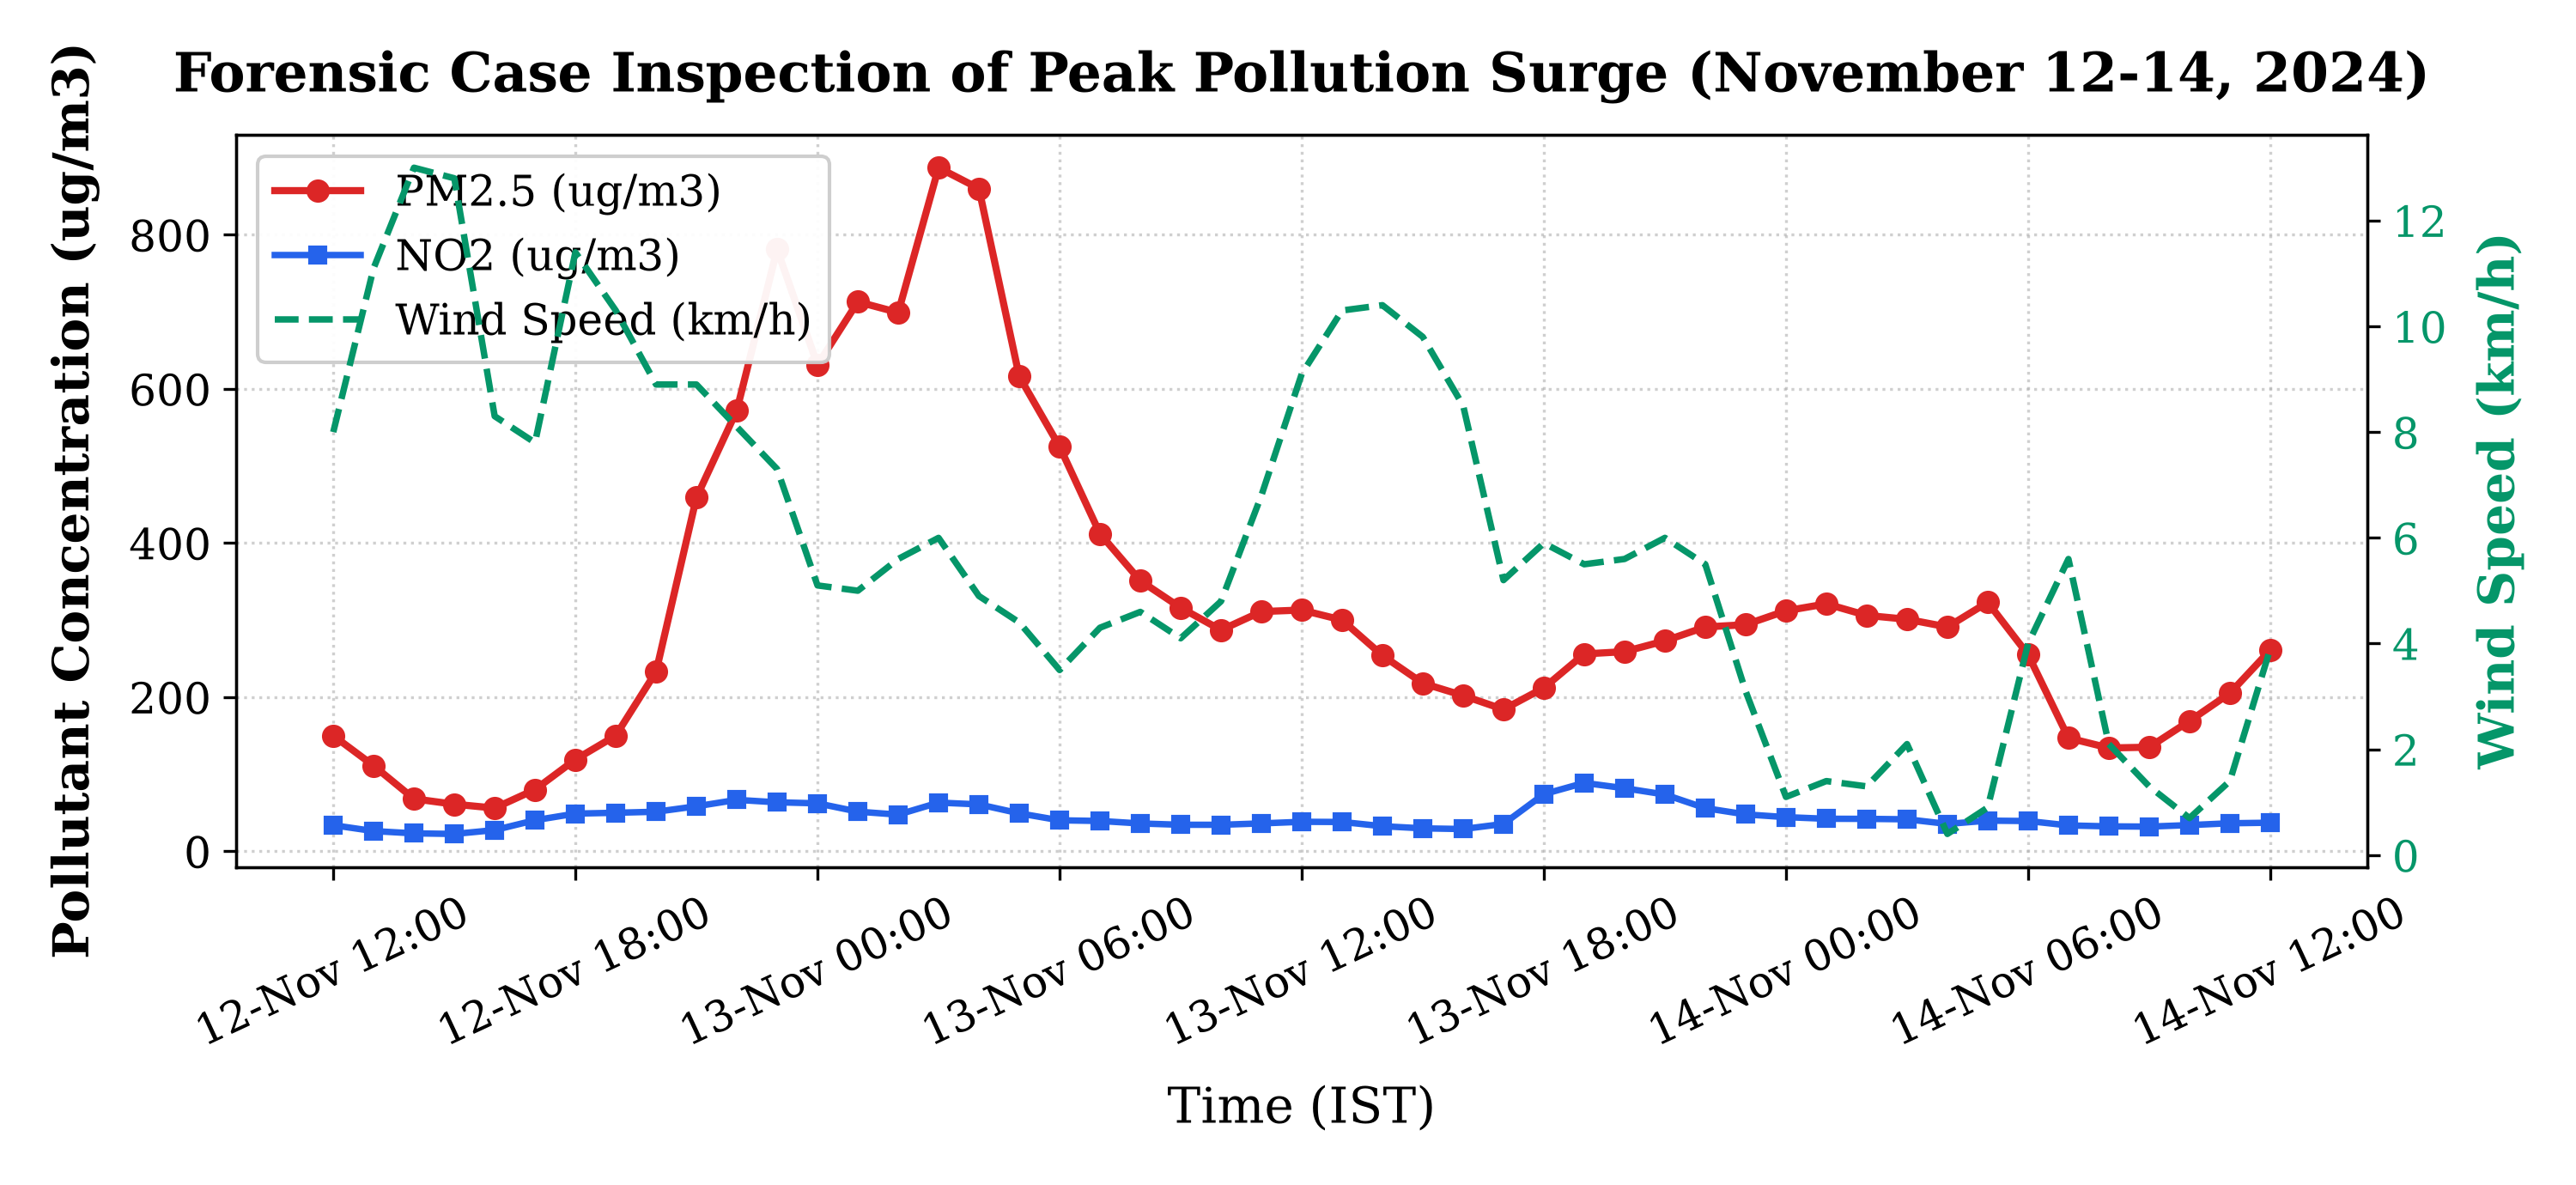
\includegraphics[width=0.90\textwidth]{figures/fig5_case_study.png}
\caption{High-resolution case study of the November 12-14 peak. $\mathrm{PM}_{2.5}$ surged to $887\,\mu\mathrm{g/m}^3$ over 5 consecutive hours accompanied by falling wind speed ($8.9 \to 5.6\,\text{km/h}$), confirming an authentic inversion episode.}
\label{fig:case}
\end{figure*}

\section{FORENSIC CASE STUDY: NOVEMBER 12-13 PEAK}

To demonstrate our system's forensic diagnostic power, we examine the highest-scoring episode in the dataset (Figure~\ref{fig:case}). On November 12, $\mathrm{PM}_{2.5}$ escalated rapidly from $150\,\mu\mathrm{g/m}^3$ at 19:00 to $781\,\mu\mathrm{g/m}^3$ by 23:00, peaking at $887\,\mu\mathrm{g/m}^3$ at 03:00 on November 13.

Our scoring model assigned this episode a score of \textbf{45 (Watch)}, activating both the Extreme Flag (35 pts) and Disagreement Flag (10 pts, as $\mathrm{NO}_2$ rose moderately to $63\,\mu\mathrm{g/m}^3$). Crucially, our system avoided classifying this as ``Suspicious'' (erroneous). As revealed by dual-axis telemetry (Figure~\ref{fig:weather}), wind speeds decelerated from $10.3\,\text{km/h}$ down to $5.1\,\text{km/h}$, indicating a shallow nocturnal boundary layer inversion trapping ground-level smoke. Furthermore, the elevation persisted across 6 consecutive hours. An electrical artifact or sensor drop would exhibit an instantaneous single-hour spike returning immediately to baseline. Our model accurately discriminated physical stagnation from instrument failure.

\section{INDIVIDUAL CONTRIBUTIONS}

Workload was partitioned across four specialized technical domains:
\begin{itemize}
  \setlength{\itemsep}{1.5pt}
  \item \textbf{Pulkit Kumar} (Department of Electrical Engineering, Reg. No: [\;\rule{1.8cm}{0.4pt}\;]): Formulated the multi-criteria mathematical scoring framework (Section 5). Led the analytical post-mortem diagnosing the affine metric compression effect (Section 7), proving why relative percentage thresholds compress under linear offsets. Implemented the software architecture, modular CLI interface, and verified $\mathcal{O}(1)$ streaming algorithmic complexity.
  \item \textbf{Vijayalakshmi AL} (Department of Electrical Engineering, Reg. No: [\;\rule{1.8cm}{0.4pt}\;]): Designed the robust non-parametric feature engineering pipeline (Section 4). Formulated the Median/IQR scaling formulation to circumvent outlier corruption. Engineered the 6-hour backward-shifted rolling median and rolling MAD algorithms, establishing the theoretical necessity of \texttt{.shift(1)} for target leakage prevention. Delivered final synthesis and conclusions.
  \item \textbf{Anant Prasad} (Department of Electrical Engineering, Reg. No: [\;\rule{1.8cm}{0.4pt}\;]): Architected the automated data acquisition pipelines interfacing the XKDR Forum CPCB API and Open-Meteo ERA5 weather API (Section 3). Enforced IST temporal synchronization across asynchronous feeds. Established and defended the Zero-Imputation Policy for anomaly screening hygiene, and constructed the cached offline execution harness.
  \item \textbf{Rama Sridhrut} (Department of Electrical Engineering, Reg. No: [\;\rule{1.8cm}{0.4pt}\;]): Directed exploratory data analysis, visual storytelling, and graphical layout (Section 6). Built the dual-axis meteorological visualization and severity-versus-suspicion diagnostics. Executed the forensic case investigation of the November 12-13 peak episode (Section 8), demonstrating the physical distinction between atmospheric stagnation and hardware glitches.
\end{itemize}

\section{LIMITATIONS AND FUTURE WORK}

We explicitly document three engineering tradeoffs:
\begin{enumerate}
  \setlength{\itemsep}{1pt}
  \item \emph{Spatial Isolation:} Evaluating a single station cannot leverage spatial consensus across neighboring monitors (e.g., Jahangirpuri, Wazirpur). Future work will incorporate spatial Kriging interpolation.
  \item \emph{Reanalysis Granularity:} ERA5 weather represents $30\,\text{km}$ gridded reanalysis rather than micro-scale rooftop conditions.
  \item \emph{Threshold Adaptation:} Future iterations will employ rolling quantile cutoffs based on the robust jump score: $\text{JumpScore}(t) = \frac{|\mathrm{Index}(t) - \tilde{M}_{6\mathrm{h}}(t)|}{\mathrm{MAD}_{6\mathrm{h}}(t) + 1}$. Thresholding at the 99th percentile ($>14.8$) naturally scales across transformed coordinate spaces.
\end{enumerate}

\section{CONCLUSION}

This project establishes that an extreme pollution observation and an anomalous measurement are distinct scientific questions. By combining robust non-parametric statistics, leakage-free rolling baselines, and meteorological dispersion context, our Python framework delivers an explainable, auditable screening tool for air quality informatics. Transforming unexpected empirical findings into mathematical insights demonstrates true data science rigor.

\subsubsection*{References}
\begin{enumerate}
  \setlength{\itemsep}{1pt}
  \footnotesize
  \item D. C. Montgomery and G. C. Runger, \emph{Applied Statistics and Probability for Engineers}, 5th ed. John Wiley \& Sons, 2011.
  \item J. L. Devore, \emph{Probability and Statistics for Engineering and the Sciences}, 8th ed. Cengage Learning, 2011.
  \item G. J. Myatt and W. P. Johnson, \emph{Making Sense of Data I: A Practical Guide to Exploratory Data Analysis and Data Mining}, 2nd ed. John Wiley \& Sons, 2014.
  \item Central Pollution Control Board (CPCB), ``Continuous Ambient Air Quality Monitoring (CAAQM) Network Technical Guidelines,'' MoEFCC, Govt. of India, 2024.
  \item XKDR Forum, ``India Air Quality Database Public API Documentation,'' \url{https://airquality.xkdr.org/}, 2024.
  \item Open-Meteo, ``ECMWF ERA5 Historical Weather Reanalysis API Documentation,'' \url{https://open-meteo.com/en/docs/historical-weather-api}, 2024.
  \item EMC Education Services, \emph{Data Science \& Big Data Analytics: Discovering, Analyzing, Visualizing and Presenting Data}. John Wiley \& Sons, 2015.
\end{enumerate}

\end{document}
